% Fields Medal Laureates - Beamer Presentation (1936–2026)
% Compact tabular layout: one laureate per row, similar to article version
% Compile with: xelatex fields_medal_laureates_beamer.tex

\documentclass[aspectratio=169,9pt]{beamer}

% ---- Theme ----
\usetheme{default}
\usecolortheme{default}
\setbeamertemplate{navigation symbols}{}
\setbeamertemplate{footline}{%
  \hfill{\tiny\color{mutedgray}\insertframenumber/\inserttotalframenumber}\hspace*{6pt}\vspace{4pt}%
}
\setbeamertemplate{frametitle}{%
  \vspace{4pt}%
  \noindent\hspace*{8pt}{\large\bfseries\color{headerblue}\insertframetitle}%
  \hfill
  \raisebox{-2pt}{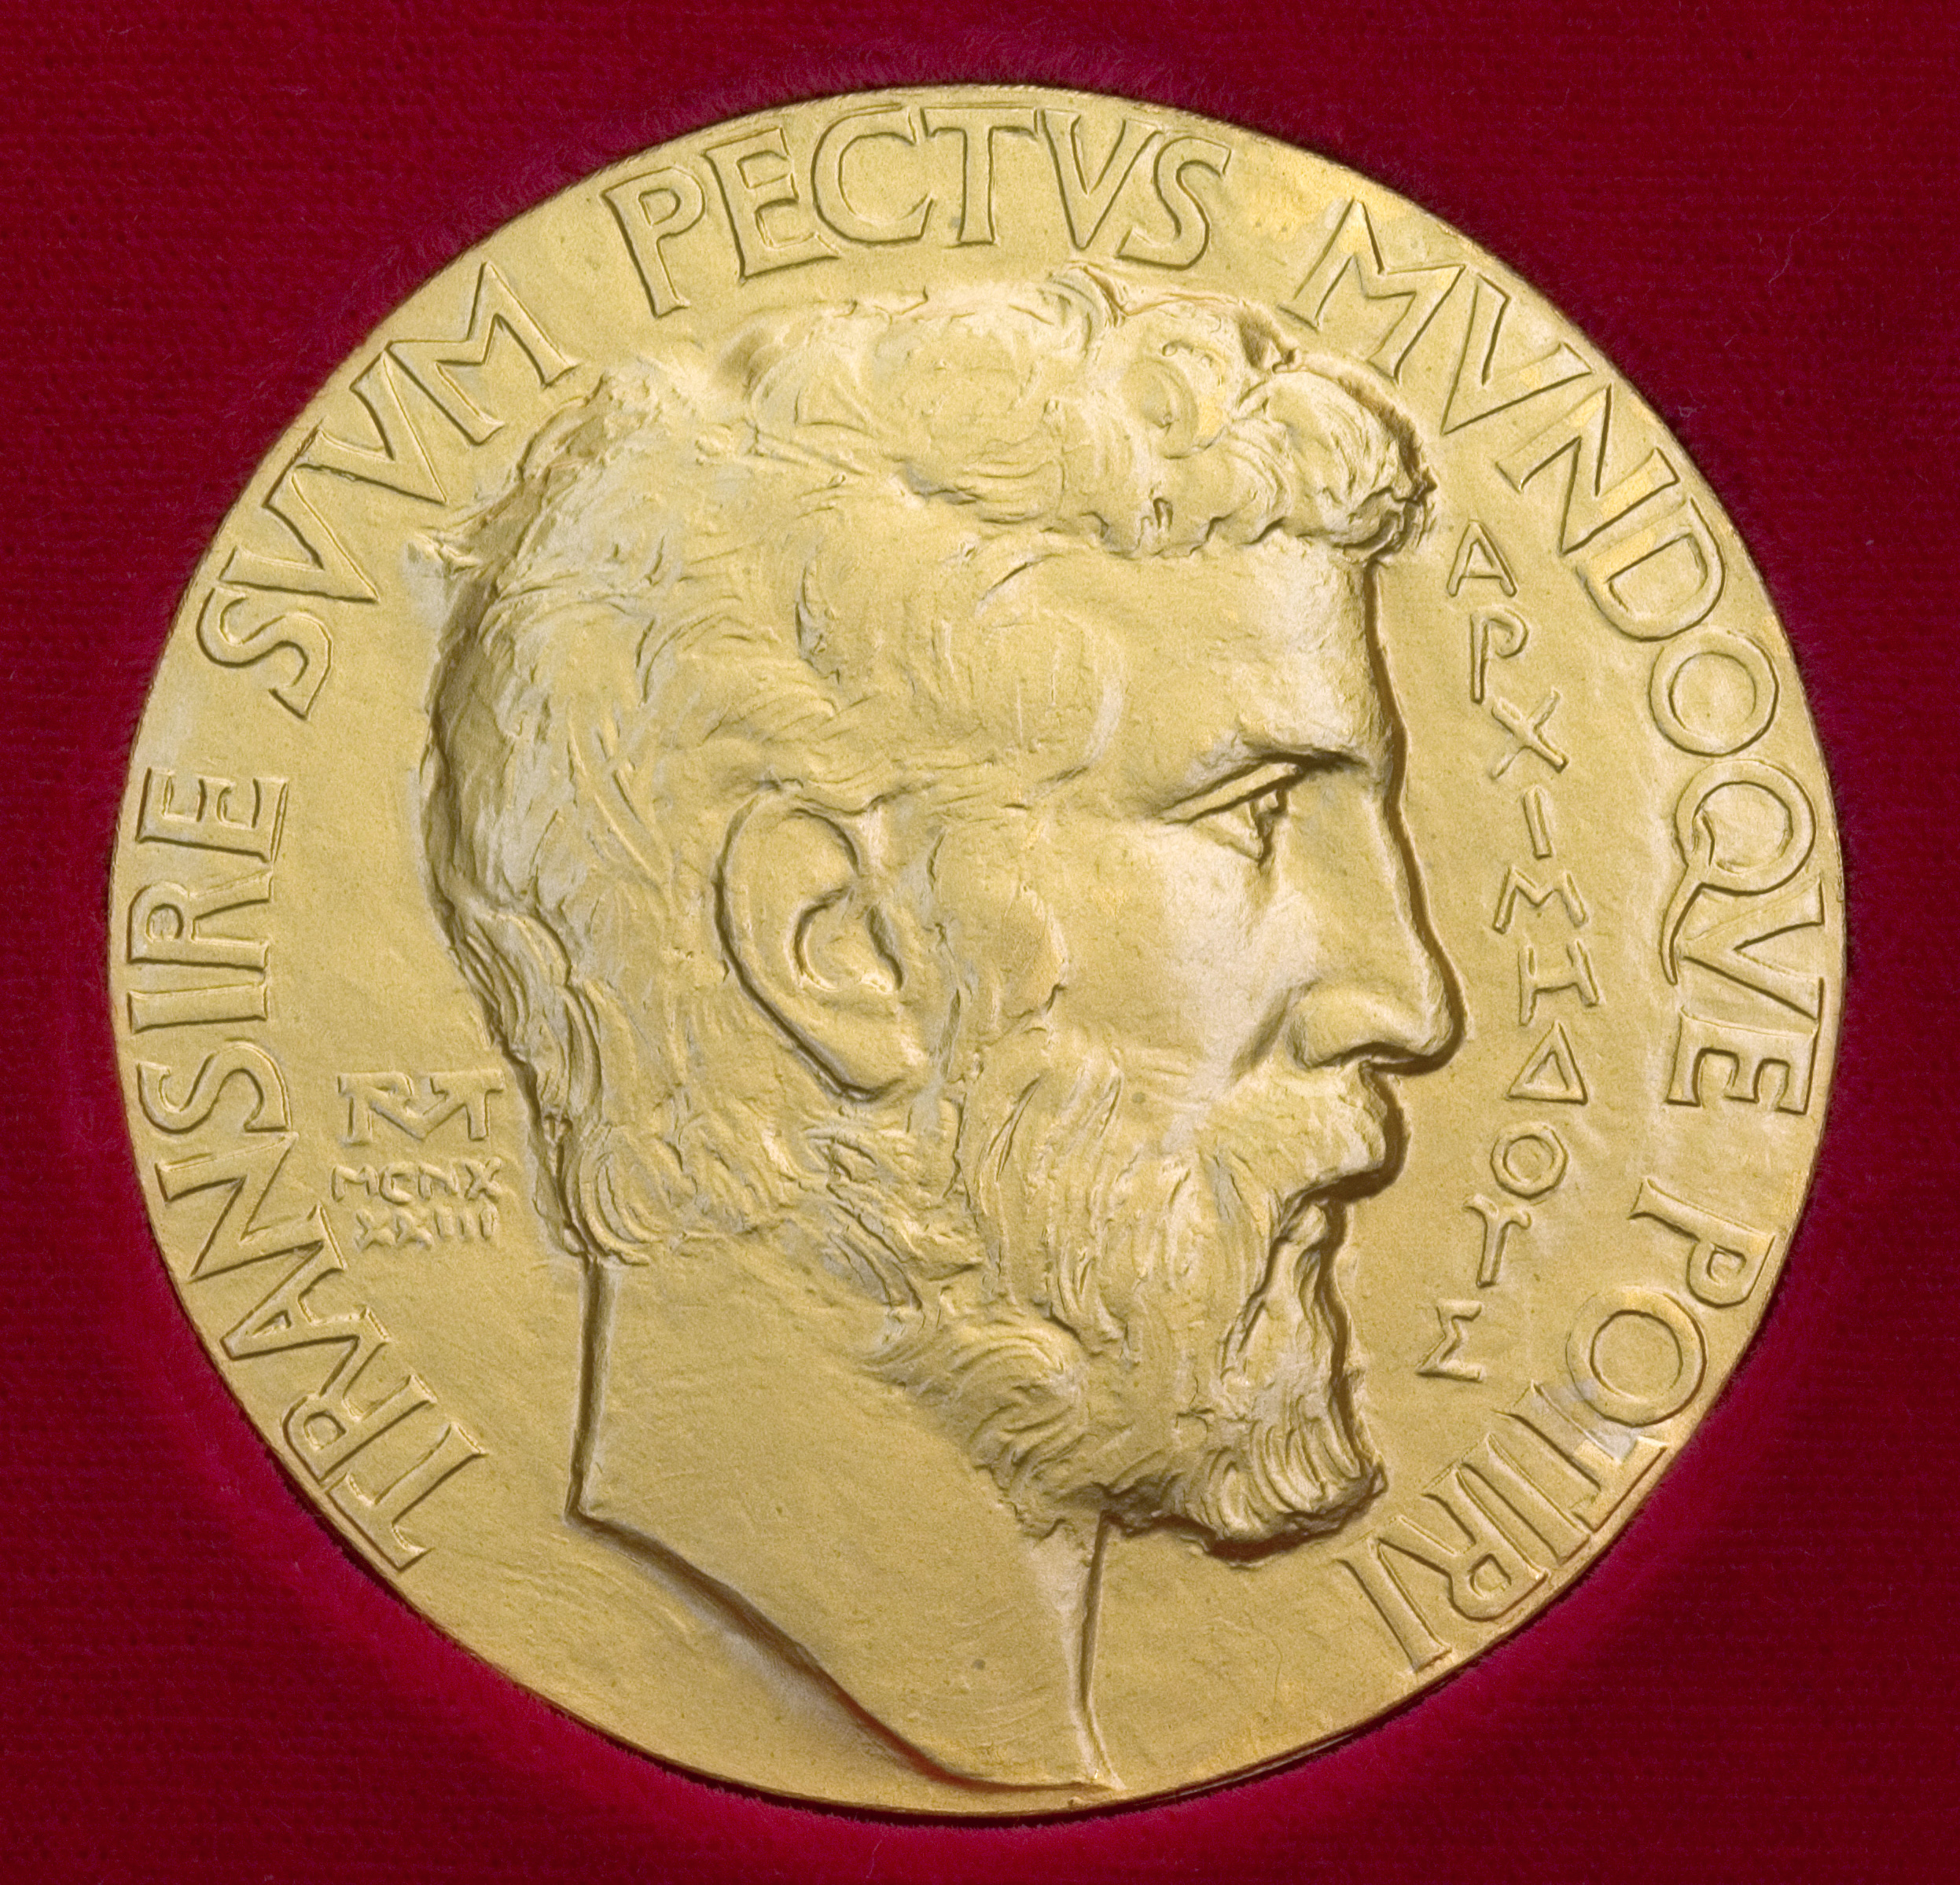
\includegraphics[height=0.7cm]{cover/FieldsMedalFront_hires.jpg}}%
  \hspace{4pt}%
  \raisebox{-2pt}{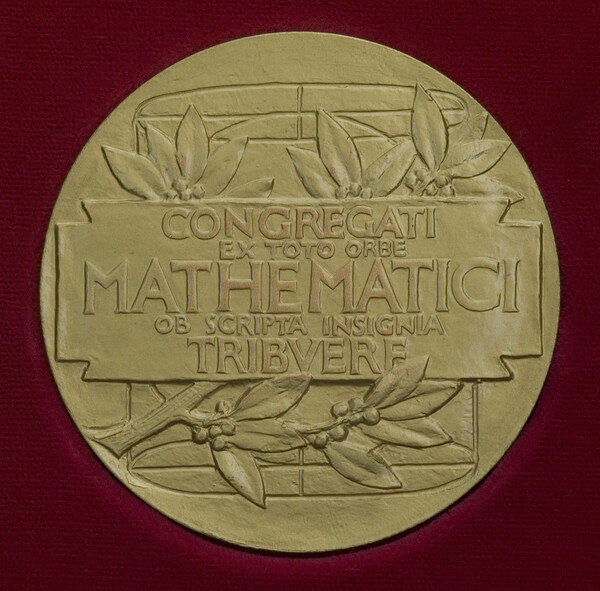
\includegraphics[height=0.7cm]{cover/FieldsMedalBack_600px.jpg}}%
  \hfill
  \hspace{8pt}%
  \vspace{2pt}%
  \par\noindent\hspace*{8pt}\textcolor{headerbg}{\rule{0.95\textwidth}{0.6pt}}%
  \vspace{-2pt}%
}

% ---- Fonts & Language ----
\usepackage{fontspec}
\usepackage{xeCJK}
\setCJKmainfont{PingFang SC}[BoldFont=PingFang SC Semibold]
\setCJKsansfont{PingFang SC}
\setmainfont{Helvetica Neue}[BoldFont=Helvetica Neue Bold]
\setsansfont{Helvetica Neue}

% ---- Packages ----
\usepackage{booktabs}
\usepackage{array}
\usepackage{tikz}
\usepackage{amssymb}
\usepackage{colortbl}
\usepackage{graphicx}

% ---- Colors ----
\definecolor{headerblue}{RGB}{41,65,122}
\definecolor{headerbg}{RGB}{200,215,240}
\definecolor{yearcolor}{RGB}{180,50,50}
\definecolor{fieldcolor}{RGB}{30,100,60}
\definecolor{mutedgray}{RGB}{100,100,100}
\definecolor{wolfcolor}{RGB}{180,120,0}
\definecolor{slidebg}{RGB}{253,254,255}
\definecolor{rowalt}{RGB}{243,247,252}
% ---- Per-award brand colors (match math_awards_allinone) ----
\definecolor{wolfclr}{RGB}{180,120,0}     % Wolf   — 金棕
\definecolor{abelclr}{RGB}{150,40,90}     % Abel   — 紫红
\definecolor{chernclr}{RGB}{15,110,92}    % Chern  — 翡翠绿

% ---- Beamer Colors ----
\setbeamercolor{background canvas}{bg=slidebg}
\setbeamercolor{title}{fg=headerblue}

% ---- Custom Commands ----
% 奖项徽标：追加在姓名后，标注该得主还获得的其他顶级奖项
\newcommand{\wolfbadge}{\textsuperscript{\normalfont\tiny\color{wolfclr}$\bigstar$\kern-0.5pt W}}
\newcommand{\abelbadge}{\textsuperscript{\normalfont\tiny\color{abelclr}$\blacktriangle$\kern-0.5pt A}}
\newcommand{\chernbadge}{\textsuperscript{\normalfont\tiny\color{chernclr}$\blacksquare$\kern-0.5pt C}}

% Table row for a laureate
% #1=Name(+badges), #2=Year(age), #3=Birth-Death, #4=Nationality, #5=Institution, #6=Field
% Name cell carries a \cn{中文名} suffix rendered on its own line in muted gray.
\newcommand{\cn}[1]{\newline{\scriptsize\color{mutedgray}#1}}
\newcommand{\lrow}[6]{%
  {\bfseries\color{headerblue}#1} & {\color{yearcolor}#2} & {#3} & {#4} & {\scriptsize #5} & {\scriptsize\color{fieldcolor}#6} \\[2.5pt]
}

% Congress section header inside table
\newcommand{\congressrow}[2]{%
  \rowcolor{headerbg}
  \multicolumn{6}{l}{\raisebox{0pt}[1.1em][0.3em]{\bfseries\color{yearcolor}\normalsize #1 \color{mutedgray}\small\enspace #2}} \\[0.5pt]
}

% ---- Document ----
\begin{document}

% ============================================================
% Title Slide
% ============================================================
\begin{frame}
\vfill
\begin{center}
  {\Huge\bfseries\color{headerblue} 菲尔兹奖获奖者名录}\\[8pt]
  {\Large\color{headerblue} Fields Medal Laureates}\\[6pt]
  {\normalsize\color{mutedgray} 1936–2026 · 21 届 · 68 位获奖者}\\[12pt]
  {\small\color{mutedgray} 按国际数学家大会届次排列}\\[8pt]
  {\footnotesize 交叉获奖标注：%
    {\color{wolfclr}$\bigstar$W} 沃尔夫奖\quad
    {\color{abelclr}$\blacktriangle$A} 阿贝尔奖\quad
    {\color{chernclr}$\blacksquare$C} 陈省身奖章}
\end{center}
\vspace{12pt}
\begin{columns}[c]
\begin{column}{0.48\textwidth}
  \centering
  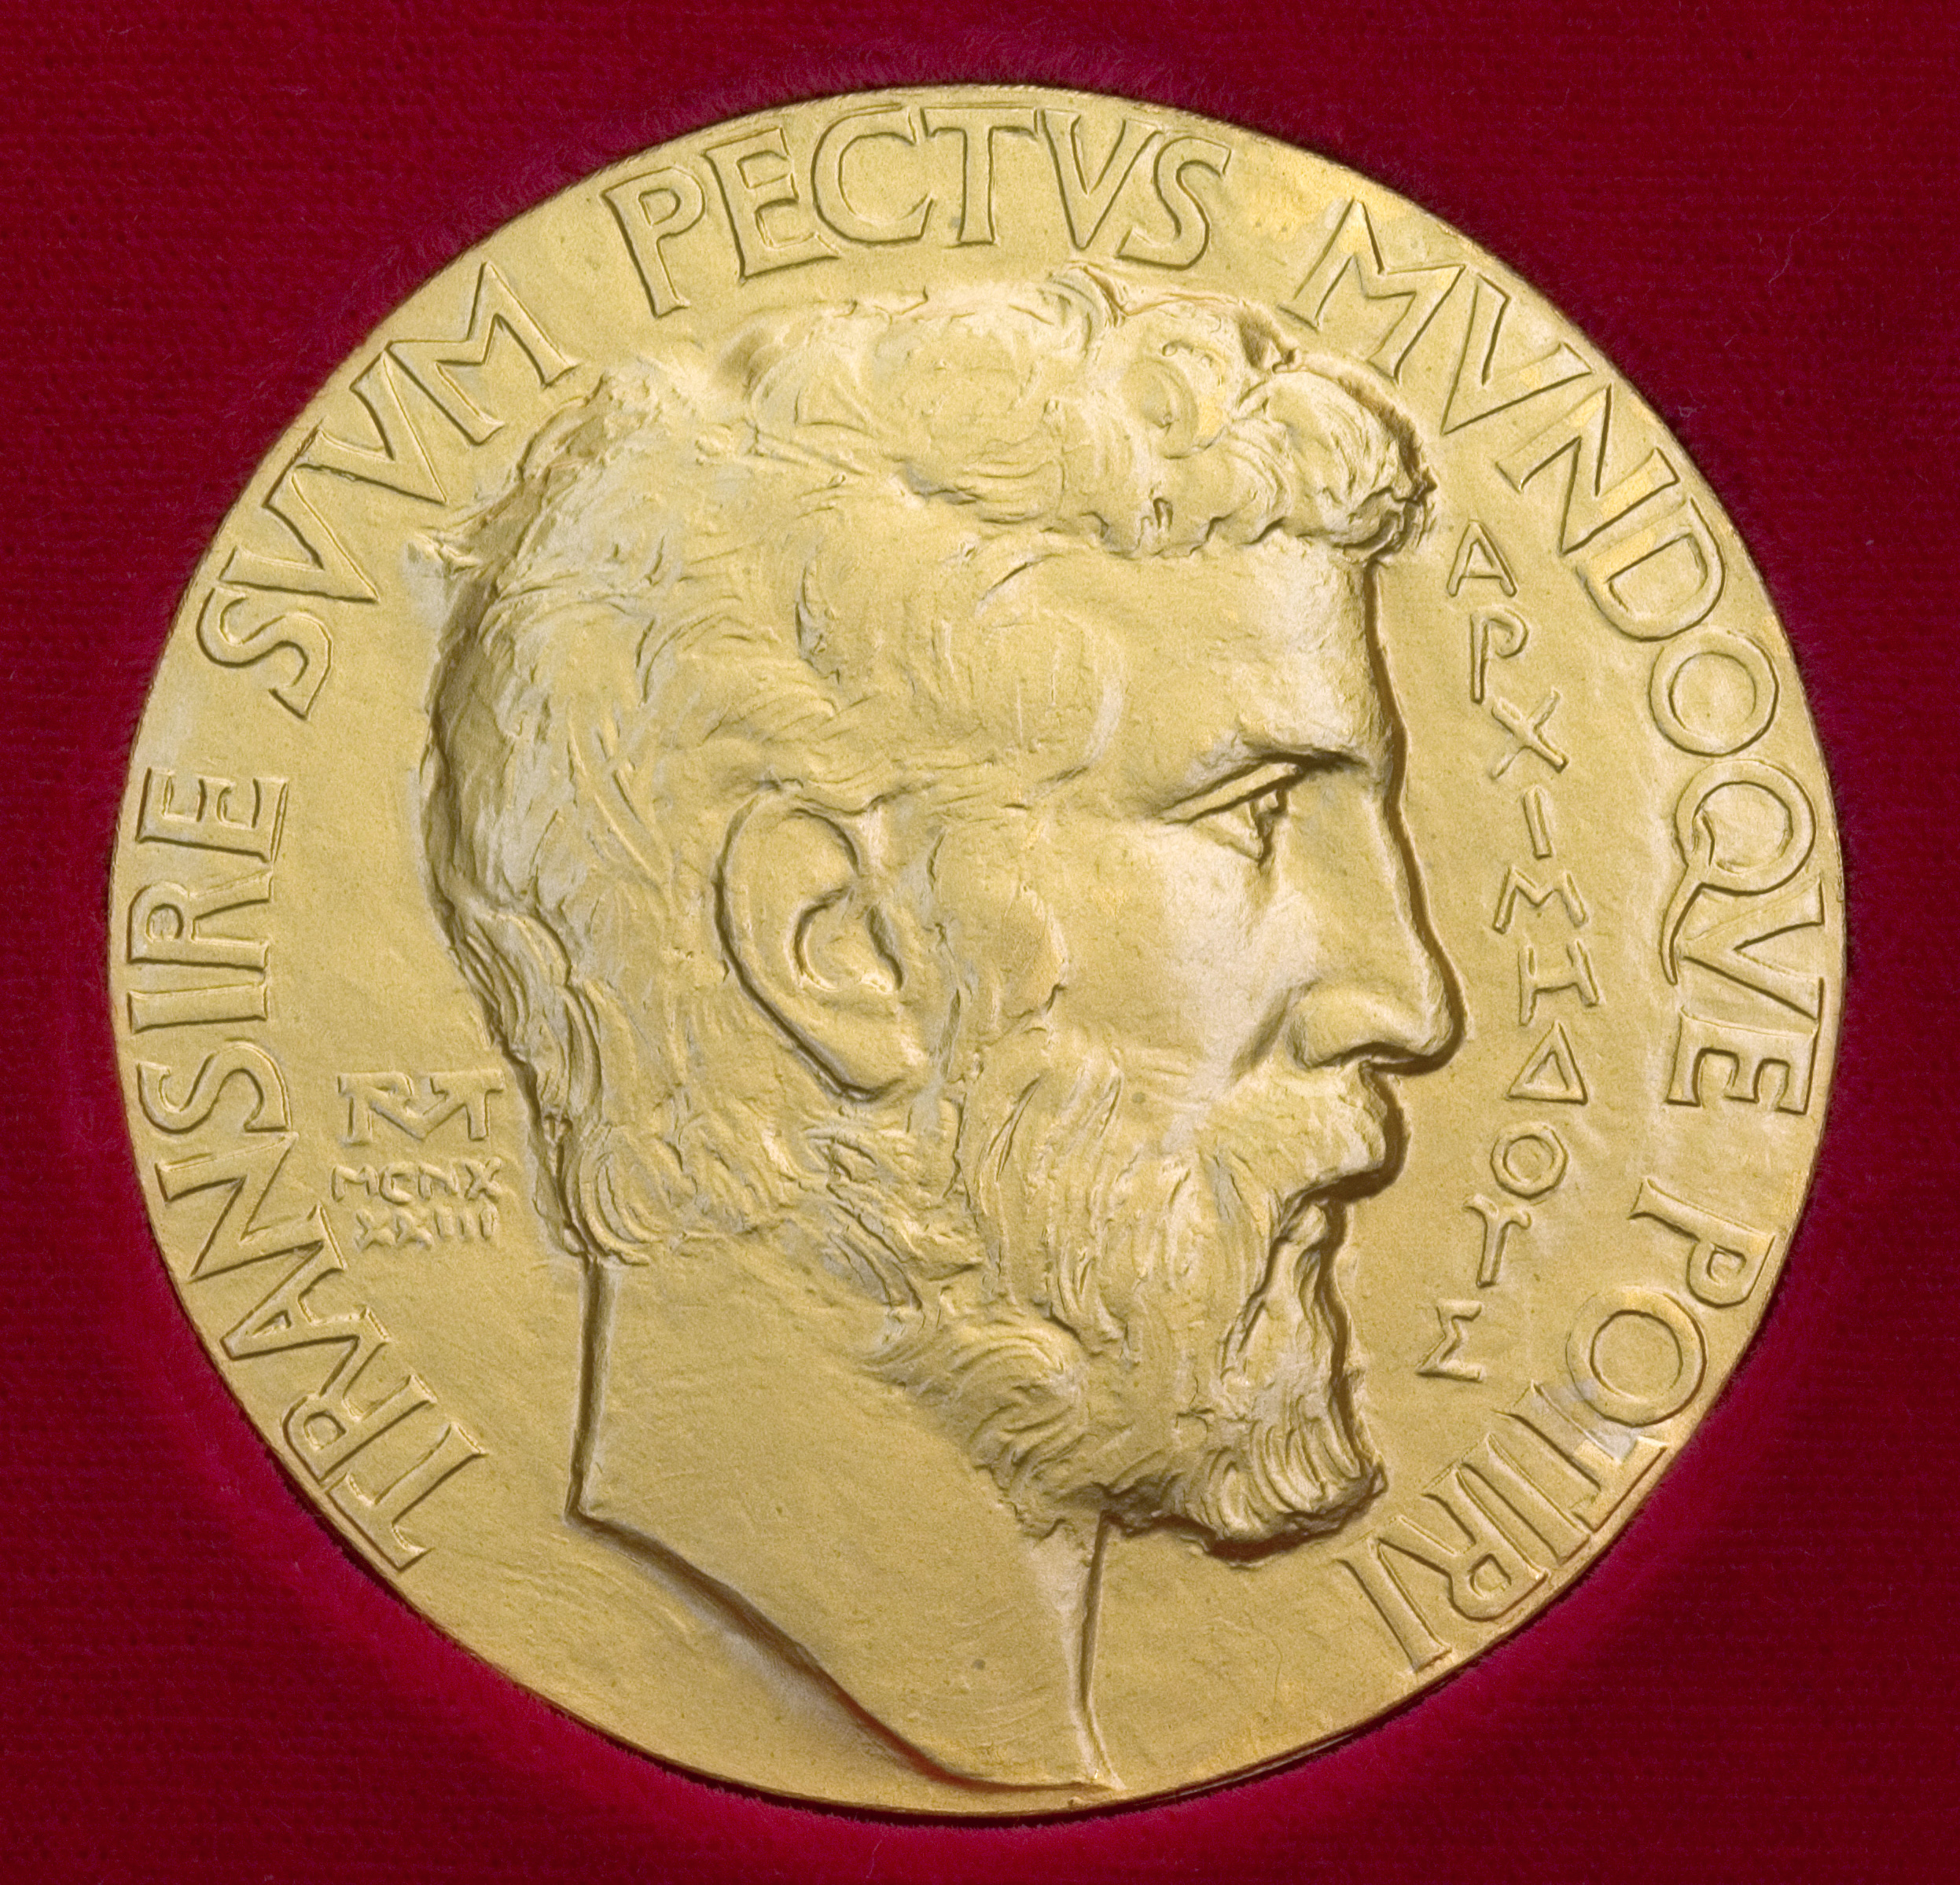
\includegraphics[height=3.5cm]{cover/FieldsMedalFront_hires.jpg}\\[4pt]
  {\tiny\color{mutedgray} 正面 · Archimedes}
\end{column}
\begin{column}{0.48\textwidth}
  \centering
  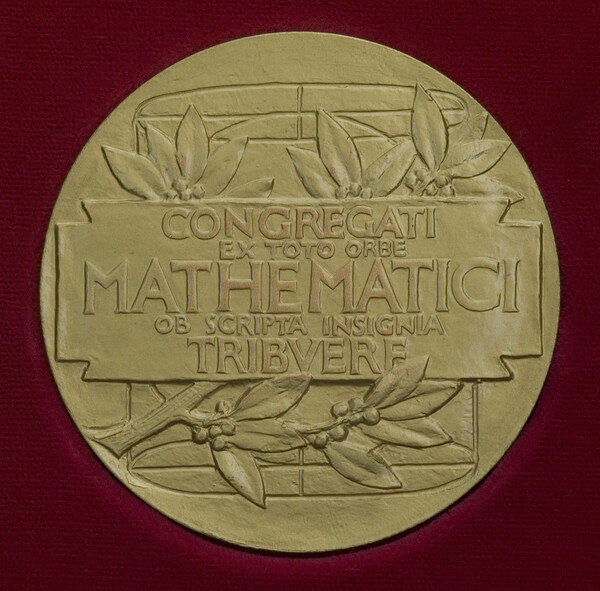
\includegraphics[height=3.5cm]{cover/FieldsMedalBack_600px.jpg}\\[4pt]
  {\tiny\color{mutedgray} 背面 · Laureate's sphere}
\end{column}
\end{columns}
\vfill
\end{frame}

% ============================================================
% Table slide 1: 1936–1954
% ============================================================
\begin{frame}{1936–1954}
\vspace{-2pt}
\centering
\scriptsize
\begin{tabular}{@{}
  >{\raggedright}m{3.5cm}
  >{\centering}m{0.85cm}
  >{\centering}m{1.1cm}
  >{\raggedright}m{1.2cm}
  >{\raggedright}m{2.3cm}
  >{\raggedright\arraybackslash}m{2.9cm}
@{}}
\toprule
\rowcolor{headerbg}
\textbf{姓名} & \textbf{获奖(龄)} & \textbf{生卒} & \textbf{国籍} & \textbf{机构} & \textbf{研究领域} \\
\midrule
\congressrow{1936}{奥斯陆 Oslo}
\lrow{Lars Ahlfors\wolfbadge\cn{拉尔斯·阿尔福斯}}{1936(29)}{1907–1996}{芬兰}{Harvard University}{复分析、黎曼曲面、拟共形映射}
\lrow{Jesse Douglas\cn{杰西·道格拉斯}}{1936(39)}{1897–1965}{美国}{MIT / City College of New York}{变分法、极小曲面（Plateau 问题）}
\congressrow{1950}{剑桥 Cambridge (USA)}
\lrow{Laurent Schwartz\cn{洛朗·施瓦茨}}{1950(35)}{1915–2002}{法国}{Université de Nancy}{分布理论、广义函数}
\lrow{Atle Selberg\wolfbadge\cn{阿特勒·塞尔伯格}}{1950(33)}{1917–2007}{挪威}{Institute for Advanced Study}{解析数论、筛法、素数定理}
\congressrow{1954}{阿姆斯特丹 Amsterdam}
\lrow{Kunihiko Kodaira\wolfbadge\cn{小平邦彦}}{1954(39)}{1915–1997}{日本}{Princeton University / 东京大学}{复流形、代数曲面分类、Hodge 理论}
\lrow{Jean-Pierre Serre\wolfbadge\abelbadge\cn{让-皮埃尔·塞尔}}{1954(27)}{1926–}{法国}{Collège de France}{代数拓扑、代数几何、数论}
\bottomrule
\end{tabular}
\end{frame}

% ============================================================
% Table slide 2: 1958–1962
% ============================================================
\begin{frame}{1958–1962}
\vspace{-2pt}
\centering
\scriptsize
\begin{tabular}{@{}
  >{\raggedright}m{3.5cm}
  >{\centering}m{0.85cm}
  >{\centering}m{1.1cm}
  >{\raggedright}m{1.2cm}
  >{\raggedright}m{2.3cm}
  >{\raggedright\arraybackslash}m{2.9cm}
@{}}
\toprule
\rowcolor{headerbg}
\textbf{姓名} & \textbf{获奖(龄)} & \textbf{生卒} & \textbf{国籍} & \textbf{机构} & \textbf{研究领域} \\
\midrule
\congressrow{1958}{爱丁堡 Edinburgh}
\lrow{Klaus Roth\cn{克劳斯·罗特}}{1958(33)}{1925–2015}{英国}{University College London}{丢番图逼近、数论}
\lrow{René Thom\cn{勒内·托姆}}{1958(35)}{1923–2002}{法国}{Université de Strasbourg}{配边理论、微分拓扑、突变论}
\congressrow{1962}{斯德哥尔摩 Stockholm}
\lrow{Lars Hörmander\wolfbadge\cn{拉尔斯·赫尔曼德}}{1962(31)}{1931–2012}{瑞典}{Stockholm Univ. / Lund Univ.}{线性偏微分算子、微局部分析}
\lrow{John Milnor\wolfbadge\abelbadge\cn{约翰·米尔诺}}{1962(31)}{1931–}{美国}{Princeton University}{微分拓扑、异国球面、K 理论}
\bottomrule
\end{tabular}
\end{frame}

% ============================================================
% Table slide 3: 1966
% ============================================================
\begin{frame}{1966}
\vspace{-2pt}
\centering
\scriptsize
\begin{tabular}{@{}
  >{\raggedright}m{3.5cm}
  >{\centering}m{0.85cm}
  >{\centering}m{1.1cm}
  >{\raggedright}m{1.2cm}
  >{\raggedright}m{2.3cm}
  >{\raggedright\arraybackslash}m{2.9cm}
@{}}
\toprule
\rowcolor{headerbg}
\textbf{姓名} & \textbf{获奖(龄)} & \textbf{生卒} & \textbf{国籍} & \textbf{机构} & \textbf{研究领域} \\
\midrule
\congressrow{1966}{莫斯科 Moscow}
\lrow{Michael Atiyah\abelbadge\cn{迈克尔·阿蒂亚}}{1966(37)}{1929–2019}{英国}{University of Oxford}{K 理论、Atiyah-Singer 指标定理}
\lrow{Paul Cohen\cn{保罗·科恩}}{1966(32)}{1934–2007}{美国}{Stanford University}{集合论、forcing、连续统假设}
\lrow{Alexander Grothendieck\cn{格罗滕迪克}}{1966(38)}{1928–2014}{法国}{IHÉS}{代数几何、概形、上同调}
\lrow{Stephen Smale\wolfbadge\cn{斯蒂芬·斯梅尔}}{1966(36)}{1930–}{美国}{UC Berkeley}{微分拓扑、高维庞加莱猜想}
\bottomrule
\end{tabular}
\end{frame}

% ============================================================
% Table slide 4: 1970–1974
% ============================================================
\begin{frame}{1970–1974}
\vspace{-2pt}
\centering
\scriptsize
\begin{tabular}{@{}
  >{\raggedright}m{3.5cm}
  >{\centering}m{0.85cm}
  >{\centering}m{1.1cm}
  >{\raggedright}m{1.2cm}
  >{\raggedright}m{2.3cm}
  >{\raggedright\arraybackslash}m{2.9cm}
@{}}
\toprule
\rowcolor{headerbg}
\textbf{姓名} & \textbf{获奖(龄)} & \textbf{生卒} & \textbf{国籍} & \textbf{机构} & \textbf{研究领域} \\
\midrule
\congressrow{1970}{尼斯 Nice}
\lrow{Alan Baker\cn{艾伦·贝克}}{1970(31)}{1939–2018}{英国}{University of Cambridge}{超越数论、线性形式对数}
\lrow{Heisuke Hironaka\cn{广中平祐}}{1970(39)}{1931–}{日本}{Harvard University}{代数几何、奇点消解}
\lrow{Sergei Novikov\wolfbadge\cn{谢尔盖·诺维科夫}}{1970(32)}{1938–2024}{苏联}{Moscow State University}{代数拓扑、Pontryagin 类}
\lrow{John G. Thompson\wolfbadge\abelbadge\cn{约翰·汤普森}}{1970(38)}{1932–}{美国}{University of Cambridge}{有限群论、奇阶定理}
\congressrow{1974}{温哥华 Vancouver}
\lrow{Enrico Bombieri\cn{恩里科·邦别里}}{1974(33)}{1940–}{意大利}{Institute for Advanced Study}{素数分布、多复变、极小曲面}
\lrow{David Mumford\wolfbadge\cn{大卫·芒福德}}{1974(37)}{1937–}{美国}{Harvard University}{代数几何、模空间、不变量理论}
\bottomrule
\end{tabular}
\end{frame}

% ============================================================
% Table slide 5: 1978
% ============================================================
\begin{frame}{1978}
\vspace{-2pt}
\centering
\scriptsize
\begin{tabular}{@{}
  >{\raggedright}m{3.5cm}
  >{\centering}m{0.85cm}
  >{\centering}m{1.1cm}
  >{\raggedright}m{1.2cm}
  >{\raggedright}m{2.3cm}
  >{\raggedright\arraybackslash}m{2.9cm}
@{}}
\toprule
\rowcolor{headerbg}
\textbf{姓名} & \textbf{获奖(龄)} & \textbf{生卒} & \textbf{国籍} & \textbf{机构} & \textbf{研究领域} \\
\midrule
\congressrow{1978}{赫尔辛基 Helsinki}
\lrow{Pierre Deligne\wolfbadge\abelbadge\cn{皮埃尔·德利涅}}{1978(33)}{1944–}{比利时}{IHÉS / IAS}{代数几何、Weil 猜想、Hodge 理论}
\lrow{Charles Fefferman\wolfbadge\cn{查尔斯·费弗曼}}{1978(29)}{1949–}{美国}{Princeton University}{多复变、调和分析}
\lrow{Grigory Margulis\wolfbadge\abelbadge\cn{格里戈里·马尔古利斯}}{1978(32)}{1946–}{苏联}{Yale University}{Lie 群格、刚性理论、遍历理论}
\lrow{Daniel Quillen\cn{丹尼尔·奎伦}}{1978(38)}{1940–2011}{美国}{MIT / University of Oxford}{代数 K 理论、同伦理论}
\bottomrule
\end{tabular}
\end{frame}

% ============================================================
% Table slide 6: 1982–1986
% ============================================================
\begin{frame}{1982–1986}
\vspace{-2pt}
\centering
\scriptsize
\begin{tabular}{@{}
  >{\raggedright}m{3.5cm}
  >{\centering}m{0.85cm}
  >{\centering}m{1.1cm}
  >{\raggedright}m{1.2cm}
  >{\raggedright}m{2.3cm}
  >{\raggedright\arraybackslash}m{2.9cm}
@{}}
\toprule
\rowcolor{headerbg}
\textbf{姓名} & \textbf{获奖(龄)} & \textbf{生卒} & \textbf{国籍} & \textbf{机构} & \textbf{研究领域} \\
\midrule
\congressrow{1982}{华沙 Warsaw}
\lrow{Alain Connes\cn{阿兰·孔涅}}{1982(35)}{1947–}{法国}{IHÉS / Collège de France}{算子代数、非交换几何}
\lrow{William Thurston\cn{威廉·瑟斯顿}}{1982(35)}{1946–2012}{美国}{Princeton University}{三维流形几何化、双曲几何}
\lrow{S.-T. Yau\wolfbadge\cn{丘成桐}}{1982(33)}{1949–}{美国/中国}{Harvard / 清华大学}{微分几何、Calabi 猜想、几何分析}
\congressrow{1986}{伯克利 Berkeley}
\lrow{Simon Donaldson\wolfbadge\cn{西蒙·唐纳森}}{1986(29)}{1957–}{英国}{Oxford / Imperial College}{四维流形、规范理论}
\lrow{Gerd Faltings\abelbadge\cn{格尔德·法尔廷斯}}{1986(32)}{1954–}{德国}{Max Planck Institute, Bonn}{算术代数几何、Mordell 猜想}
\lrow{Michael Freedman\cn{迈克尔·弗里德曼}}{1986(35)}{1951–}{美国}{UC San Diego / Microsoft}{四维拓扑、庞加莱猜想（拓扑版）}
\bottomrule
\end{tabular}
\end{frame}

% ============================================================
% Table slide 7: 1990
% ============================================================
\begin{frame}{1990}
\vspace{-2pt}
\centering
\scriptsize
\begin{tabular}{@{}
  >{\raggedright}m{3.5cm}
  >{\centering}m{0.85cm}
  >{\centering}m{1.1cm}
  >{\raggedright}m{1.2cm}
  >{\raggedright}m{2.3cm}
  >{\raggedright\arraybackslash}m{2.9cm}
@{}}
\toprule
\rowcolor{headerbg}
\textbf{姓名} & \textbf{获奖(龄)} & \textbf{生卒} & \textbf{国籍} & \textbf{机构} & \textbf{研究领域} \\
\midrule
\congressrow{1990}{京都 Kyoto}
\lrow{Vladimir Drinfeld\wolfbadge\cn{弗拉基米尔·德林费尔德}}{1990(36)}{1954–}{苏联/美国}{University of Chicago}{Langlands 纲领、量子群}
\lrow{Vaughan Jones\cn{沃恩·琼斯}}{1990(38)}{1952–2020}{新西兰}{UC Berkeley}{von Neumann 代数、Jones 多项式}
\lrow{Shigefumi Mori\cn{森重文}}{1990(39)}{1951–}{日本}{Kyoto University}{代数几何、极小模型纲领}
\lrow{Edward Witten\cn{爱德华·威滕}}{1990(38)}{1951–}{美国}{Institute for Advanced Study}{数学物理、量子场论与几何}
\bottomrule
\end{tabular}
\end{frame}

% ============================================================
% Table slide 8: 1994
% ============================================================
\begin{frame}{1994}
\vspace{-2pt}
\centering
\scriptsize
\begin{tabular}{@{}
  >{\raggedright}m{3.5cm}
  >{\centering}m{0.85cm}
  >{\centering}m{1.1cm}
  >{\raggedright}m{1.2cm}
  >{\raggedright}m{2.3cm}
  >{\raggedright\arraybackslash}m{2.9cm}
@{}}
\toprule
\rowcolor{headerbg}
\textbf{姓名} & \textbf{获奖(龄)} & \textbf{生卒} & \textbf{国籍} & \textbf{机构} & \textbf{研究领域} \\
\midrule
\congressrow{1994}{苏黎世 Zürich}
\lrow{Jean Bourgain\cn{让·布尔甘}}{1994(39)}{1954–2018}{比利时}{IHÉS / IAS}{Banach 空间、调和分析、组合数论}
\lrow{Pierre-Louis Lions\cn{皮埃尔-路易·利翁斯}}{1994(38)}{1956–}{法国}{Collège de France}{非线性 PDE、最优控制、黏性解}
\lrow{J.-C. Yoccoz\cn{让-克里斯托夫·约科兹}}{1994(37)}{1957–2016}{法国}{Collège de France}{动力系统、小除数问题}
\lrow{Efim Zelmanov\cn{叶菲姆·泽尔曼诺夫}}{1994(39)}{1955–}{俄罗斯/美国}{UC San Diego}{代数、限制 Burnside 问题}
\bottomrule
\end{tabular}
\end{frame}

% ============================================================
% Table slide 9: 1998–2002
% ============================================================
\begin{frame}{1998–2002}
\vspace{-2pt}
\centering
\scriptsize
\begin{tabular}{@{}
  >{\raggedright}m{3.5cm}
  >{\centering}m{0.85cm}
  >{\centering}m{1.1cm}
  >{\raggedright}m{1.2cm}
  >{\raggedright}m{2.3cm}
  >{\raggedright\arraybackslash}m{2.9cm}
@{}}
\toprule
\rowcolor{headerbg}
\textbf{姓名} & \textbf{获奖(龄)} & \textbf{生卒} & \textbf{国籍} & \textbf{机构} & \textbf{研究领域} \\
\midrule
\congressrow{1998}{柏林 Berlin}
\lrow{Richard Borcherds\cn{理查德·博彻兹}}{1998(38)}{1959–}{英国}{UC Berkeley}{顶点代数、怪兽月光猜想}
\lrow{Timothy Gowers\cn{蒂莫西·高尔斯}}{1998(34)}{1963–}{英国}{University of Cambridge}{泛函分析、组合数学}
\lrow{Maxim Kontsevich\cn{马克西姆·孔采维奇}}{1998(34)}{1964–}{俄罗斯/法国}{IHÉS}{数学物理、Witten 猜想、形变量子化}
\lrow{Curtis T. McMullen\cn{柯蒂斯·麦克马伦}}{1998(40)}{1958–}{美国}{Harvard University}{复动力系统、Teichmüller 理论}
\congressrow{2002}{北京 Beijing}
\lrow{Laurent Lafforgue\cn{洛朗·拉福格}}{2002(36)}{1966–}{法国}{IHÉS}{Langlands 对应（函数域）}
\lrow{Vladimir Voevodsky\cn{沃埃沃德斯基}}{2002(36)}{1966–2017}{俄罗斯}{Institute for Advanced Study}{动机上同调、A$^1$ 同伦理论}
\bottomrule
\end{tabular}
\end{frame}

% ============================================================
% Table slide 10: 2006
% ============================================================
\begin{frame}{2006}
\vspace{-2pt}
\centering
\scriptsize
\begin{tabular}{@{}
  >{\raggedright}m{3.5cm}
  >{\centering}m{0.85cm}
  >{\centering}m{1.1cm}
  >{\raggedright}m{1.2cm}
  >{\raggedright}m{2.3cm}
  >{\raggedright\arraybackslash}m{2.9cm}
@{}}
\toprule
\rowcolor{headerbg}
\textbf{姓名} & \textbf{获奖(龄)} & \textbf{生卒} & \textbf{国籍} & \textbf{机构} & \textbf{研究领域} \\
\midrule
\congressrow{2006}{马德里 Madrid}
\lrow{Andrei Okounkov\cn{安德烈·奥昆科夫}}{2006(37)}{1969–}{俄罗斯/美国}{Princeton / Columbia Univ.}{表示论、随机分拆、代数几何}
\lrow{Grigori Perelman\cn{格里戈里·佩雷尔曼}}{2006(40)}{1966–}{俄罗斯}{无（拒绝领奖）}{Ricci 流、庞加莱猜想}
\lrow{Terence Tao\cn{陶哲轩}}{2006(31)}{1975–}{澳/美}{UCLA}{调和分析、PDE、加性数论}
\lrow{Wendelin Werner\cn{温德林·维尔纳}}{2006(38)}{1968–}{法国}{Univ. Paris-Sud / ETH Zürich}{概率论、SLE、二维布朗运动}
\bottomrule
\end{tabular}
\end{frame}

% ============================================================
% Table slide 11: 2010
% ============================================================
\begin{frame}{2010}
\vspace{-2pt}
\centering
\scriptsize
\begin{tabular}{@{}
  >{\raggedright}m{3.5cm}
  >{\centering}m{0.85cm}
  >{\centering}m{1.1cm}
  >{\raggedright}m{1.2cm}
  >{\raggedright}m{2.3cm}
  >{\raggedright\arraybackslash}m{2.9cm}
@{}}
\toprule
\rowcolor{headerbg}
\textbf{姓名} & \textbf{获奖(龄)} & \textbf{生卒} & \textbf{国籍} & \textbf{机构} & \textbf{研究领域} \\
\midrule
\congressrow{2010}{海得拉巴 Hyderabad}
\lrow{Elon Lindenstrauss\cn{林登施特劳斯}}{2010(40)}{1970–}{以色列}{Hebrew Univ. of Jerusalem}{遍历理论、测度刚性、数论}
\lrow{Ngô Bảo Châu\cn{吴宝珠}}{2010(38)}{1972–}{越南/法国}{Univ. Paris-Sud / Chicago}{代数几何、基本引理}
\lrow{Stanislav Smirnov\cn{斯米尔诺夫}}{2010(40)}{1970–}{俄罗斯}{Université de Genève}{统计物理、渗流共形不变性}
\lrow{Cédric Villani\cn{塞德里克·维拉尼}}{2010(37)}{1973–}{法国}{Institut Henri Poincaré}{最优传输、Boltzmann 方程}
\bottomrule
\end{tabular}
\end{frame}

% ============================================================
% Table slide 12: 2014
% ============================================================
\begin{frame}{2014}
\vspace{-2pt}
\centering
\scriptsize
\begin{tabular}{@{}
  >{\raggedright}m{3.5cm}
  >{\centering}m{0.85cm}
  >{\centering}m{1.1cm}
  >{\raggedright}m{1.2cm}
  >{\raggedright}m{2.3cm}
  >{\raggedright\arraybackslash}m{2.9cm}
@{}}
\toprule
\rowcolor{headerbg}
\textbf{姓名} & \textbf{获奖(龄)} & \textbf{生卒} & \textbf{国籍} & \textbf{机构} & \textbf{研究领域} \\
\midrule
\congressrow{2014}{首尔 Seoul}
\lrow{Artur Avila\cn{阿图尔·阿维拉}}{2014(35)}{1979–}{巴西/法国}{IMPA / Univ. Paris Diderot}{动力系统、谱理论、重整化}
\lrow{Manjul Bhargava\cn{曼朱·巴尔加瓦}}{2014(40)}{1974–}{加拿大/美国}{Princeton University}{数论、数的几何、椭圆曲线}
\lrow{Martin Hairer\cn{马丁·海雷尔}}{2014(39)}{1975–}{奥地利/英国}{Warwick / Imperial College}{随机 PDE、正则结构理论}
\lrow{Maryam Mirzakhani\cn{米尔札哈尼}}{2014(37)}{1977–2017}{伊朗}{Stanford University}{黎曼曲面模空间、双曲几何}
\bottomrule
\end{tabular}
\end{frame}

% ============================================================
% Table slide 13: 2018
% ============================================================
\begin{frame}{2018}
\vspace{-2pt}
\centering
\scriptsize
\begin{tabular}{@{}
  >{\raggedright}m{3.5cm}
  >{\centering}m{0.85cm}
  >{\centering}m{1.1cm}
  >{\raggedright}m{1.2cm}
  >{\raggedright}m{2.3cm}
  >{\raggedright\arraybackslash}m{2.9cm}
@{}}
\toprule
\rowcolor{headerbg}
\textbf{姓名} & \textbf{获奖(龄)} & \textbf{生卒} & \textbf{国籍} & \textbf{机构} & \textbf{研究领域} \\
\midrule
\congressrow{2018}{里约热内卢 Rio de Janeiro}
\lrow{Caucher Birkar\cn{考切尔·比尔卡尔}}{2018(40)}{1978–}{英国}{University of Cambridge}{代数几何、Fano 簇有界性}
\lrow{Alessio Figalli\cn{阿莱西奥·菲加利}}{2018(34)}{1984–}{意大利}{ETH Zürich}{最优传输、自由边界问题}
\lrow{Peter Scholze\cn{彼得·朔尔策}}{2018(30)}{1987–}{德国}{Bonn / Max Planck Institute}{perfectoid 空间、p-adic 几何}
\lrow{Akshay Venkatesh\cn{文卡泰什}}{2018(36)}{1981–}{澳大利亚}{Institute for Advanced Study}{数论、表示论、动力系统}
\bottomrule
\end{tabular}
\end{frame}

% ============================================================
% Table slide 14: 2022
% ============================================================
\begin{frame}{2022}
\vspace{-2pt}
\centering
\scriptsize
\begin{tabular}{@{}
  >{\raggedright}m{3.5cm}
  >{\centering}m{0.85cm}
  >{\centering}m{1.1cm}
  >{\raggedright}m{1.2cm}
  >{\raggedright}m{2.3cm}
  >{\raggedright\arraybackslash}m{2.9cm}
@{}}
\toprule
\rowcolor{headerbg}
\textbf{姓名} & \textbf{获奖(龄)} & \textbf{生卒} & \textbf{国籍} & \textbf{机构} & \textbf{研究领域} \\
\midrule
\congressrow{2022}{赫尔辛基 Helsinki}
\lrow{Hugo Duminil-Copin\cn{迪米尼-科潘}}{2022(36)}{1985–}{法国}{IHÉS / Univ. de Genève}{统计物理、相变、概率论}
\lrow{June Huh\cn{许埈珥}}{2022(39)}{1983–}{韩国/美国}{Princeton University}{组合数学、Hodge 理论、代数几何}
\lrow{James Maynard\cn{詹姆斯·梅纳德}}{2022(35)}{1987–}{英国}{University of Oxford}{解析数论、素数间隔}
\lrow{Maryna Viazovska\cn{维亚佐夫斯卡}}{2022(37)}{1984–}{乌克兰}{EPFL}{Fourier 分析、球堆积问题}
\bottomrule
\end{tabular}
\end{frame}

% ============================================================
% Table slide 15: 2026
% ============================================================
\begin{frame}{2026}
\vspace{-2pt}
\centering
\scriptsize
\begin{tabular}{@{}
  >{\raggedright}m{3.5cm}
  >{\centering}m{0.85cm}
  >{\centering}m{1.1cm}
  >{\raggedright}m{1.2cm}
  >{\raggedright}m{2.3cm}
  >{\raggedright\arraybackslash}m{2.9cm}
@{}}
\toprule
\rowcolor{headerbg}
\textbf{姓名} & \textbf{获奖(龄)} & \textbf{生卒} & \textbf{国籍} & \textbf{机构} & \textbf{研究领域} \\
\midrule
\congressrow{2026}{费城 Philadelphia}
\lrow{Yu Deng\cn{邓煜}}{2026(35)}{1990–}{中国/美国}{University of Chicago}{PDE、Boltzmann 方程推导}
\lrow{John Pardon\cn{约翰·帕登}}{2026(37)}{1989–}{美国}{Princeton University}{辛几何、Fukaya 范畴}
\lrow{Jacob Tsimerman\cn{雅各布·齐默尔曼}}{2026(38)}{1988–}{加拿大}{University of Toronto}{数论、o-minimality、算术几何}
\lrow{Hong Wang\cn{王虹}}{2026(35)}{1990–}{中国/美国}{NYU Courant Institute}{几何测度论、Kakeya 问题}
\bottomrule
\end{tabular}
\end{frame}

% ============================================================
% Summary / legend slide
% ============================================================
\begin{frame}{统计与图例}
\vspace{6pt}
\centering
\vspace{8pt}
{\footnotesize\color{mutedgray} 共 21 届 · 68 位获奖者 \quad 交叉获奖：{\color{wolfclr}$\bigstar$W} 沃尔夫奖 · {\color{abelclr}$\blacktriangle$A} 阿贝尔奖 · {\color{chernclr}$\blacksquare$C} 陈省身奖章 \quad 首位女性：Mirzakhani (2014) \quad 最年轻：Serre (27岁)}

\end{frame}

\end{document}
